
    \begin{comment}


    To perform an analysis of the results and determine if there was correlation between the number of times the mandatory conditions were met and whether or not we would classify the fault as fully functional or partially functional we examined the goodstates that we captured and then grouped all cell aware faults into eight groups depending on how many times their mandatory conditions were met. We similarly grouped faults depending on whether or not they were detected in the first set of 40,000 goodstates, the second set of 40,000 goodstates, or both sets (for the ISCAS circuits). The color bar graphs below represent the frequencies for each of the five ISCAS circuits that we used. 

    \textbf{INSERT DATA HERE}

    As we can see from the data there doesn't appear to be much correlation between the mandatory counts and whether or not a fault was purely functional. This is likely owing to the fact that random inputs were used in order to generate the goodstates instead of functional patterns. For the DES56 circuit however, we used a functional test bench, and the data is much more aligned with what we were expecting to see. 

    \textbf{INSERT DATA HERE}

    There are several interesting implications that can be drawn from this data. For instance, we can now determine which faults are the most important to test for simply by running functional simulation. These implications and their industry applications will be discussed in the conclusion. 

    \end{comment}

    To start out, we used a very basic selection criteria for predictions and observations.
    If a fault's mandatory count was greater than zero, then the fault was ``predicted'' to be a functional fault.
    Similarly, if a fault had any goodstate detections during simulation, then the fault was ``observed'' to be a functional fault.
    In future efforts we will refine this criteria and examine the resulting increases or decreases in precision.

\subsection{Mandatory Counts as Fault Classifiers}
    As mentioned in the preceding section, we have analyzed two particular circuits during this research. 
    The first of which was an ISCAS 89' benchmark circuit called ``s9234''. 
    The circuit contains sequential logic, and 9,234 logic gates,. 
    Other than those two facts, we did not determine the true function of the circuit. 
    This allowed us to emulate testing procedure when the function of a circuit is unknown. 
    After performing the experiment described above we determined that there were 1,034 detectable cell aware faults in the circuit. 
    We claim that a fault is predicted to be functional if the mandatory count for that fault is greater than 0. 
    In other words, mandatory conditions predict a fault to be functional if they are detected at least once during functional simulation. 
    Similarly, we define the observance of a functional fault, if the fault was detected one or more times during goodstate fault simulation. 
    Therefore we can construct the  confusion matrix in Figure \ref{fig:confs9234} to describe the usage of mandatory conditions as a predictor when the function of a particular circuit is unknown, and is guessed by randomly stimulating the inputs during simulation. 

\begin{figure}
\caption{Confusion Matrix for s9234\label{fig:confs9234}}
\vspace{1 em}
\begin{center}
\begin{tabular}{cc|c|c|}
\cline{3-4}
& & \multicolumn{2}{ c| }{Detected} \\ \cline{3-4}
& & T & F\\ \cline{1-4}
\multicolumn{1}{ |c  }{\multirow{2}{*}{Predicted} } &
\multicolumn{1}{ |c| }{T} & 453 (TP) & 119 (FP)    \\ \cline{2-4}
\multicolumn{1}{ |c  }{}                        &
\multicolumn{1}{ |c| }{F} & 0 (FN) & 462 (TN)    \\ \cline{1-4}
\end{tabular}
\end{center}
\end{figure}

    We also calculate several statistics in Figure \ref{fig:stats9234} to determine how well mandatory counts predict in this case. 

\begin{figure}
\caption{Statistics for s9234\label{fig:stats9234}}
\vspace{1 em}
\begin{center}
\begin{tabular}{| c | c |}
\hline
Statistic &  Value \\
\hline
\hline
Precision & 79\% \\ 
\hline 
Accuracy & 88\% \\ 
\hline 
Specificity & 79\% \\ 
\hline 
Fall-out & 20.5\% \\ 
\hline
\end{tabular}
\end{center}
\end{figure}

    In summary, Mandatory conditions are really not a spectacular indicator of whether or not a fault is functional when the function of the circuit is unknown. 
    Again, in future efforts we will manipulate the prediction criteria more to determine if increasing the required mandatory count before a fault is ``predicted'' functional will have a positive effect on these statistics. 
    With the second circuit we tested however (DES56) the function was known, and we had much better results. 
    The confusion matrix for this circuit is in Figure \ref{fig:confdes} 


\begin{figure}[h!]
\caption{Confusion Matrix for DES56\label{fig:confdes}}
\vspace{1 em}
\begin{center}
\begin{tabular}{cc|c|c|}
\cline{3-4}
& & \multicolumn{2}{ c| }{Detected} \\ \cline{3-4}
& & T & F\\ \cline{1-4}
\multicolumn{1}{ |c  }{\multirow{2}{*}{Predicted} } &
\multicolumn{1}{ |c| }{T} & 461 (TP) & 2 (FP)    \\ \cline{2-4}
\multicolumn{1}{ |c  }{}                        &
\multicolumn{1}{ |c| }{F} & 0 (FN) & 14 (TN)    \\ \cline{1-4}
\end{tabular}
\end{center}
\end{figure}

    Again the statistics were calculated based on the matrix (Figure \ref{fig:statdes}), and this time we saw much better results. 

\begin{figure}[h!]
\caption{Statistics for DES56\label{fig:statdes}}
\vspace{1 em}
\begin{center}
\begin{tabular}{| c | c |}
\hline
Statistic &  Value \\
\hline
\hline
Sensitivity & 100\% \\ 
\hline
Accuracy & 99.5\% \\ 
\hline
Specificity & 87.5\% \\ 
\hline
Fall-out & 14.2\% \\ 
\hline
Precision & 99.5\% \\
\hline
\end{tabular}
\end{center}
\end{figure}
    
    We can see that this is an extremely accurate classification methodology if you know the functionality of the circuit. 
    We can calculate the $F_1$ score of the predictor as well (values closer to one represent a better classification scheme).
    The $F_1$ score for this confusion matrix is 0.997835. 
    This is a very high $F_1$ score, which again corroborates that Mandatory counts during functional simulation are excellent classifiers. 
    The final statistic produced in regards to this confusion matrix is known as Matthew's correlation coefficient. 
    This is a good segue into the next analysis of our data, as it represents only a single way that the correlation of two variables can be calculated, but specifically regards the false negative and false positive rates described by the confusion matrix. 
    Matthew's correlation coefficient is calculated to be 0.93339, again this is a very high value, which indicates that these mandatory counts are a spectacular predictor of functional faults. 

    In the future we intend to extend this analysis by increasing the mandatory count before a particular fault is predicted, and drawing an ROC to analyze if there is any increase in precision.

\subsection{Regression Analysis}

    In addition to the standard confusion matrix analysis for a predictor that was done above, we also determined the line of best fit for our data, and calculated Pearson's correlation coefficient and the $R^2$ value for our data. 
    Somewhat surprisingly, there was a high correlation for the first circuit, when using Pearson's correlation coefficient. 
    it was determined that $\rho = 0.77$ which indicates that there is a strongly positive correlation within the data. 
    This became slightly more obvious when a plot of the data as well as a linear regression line was produced. 
    This plot is shown in Figure \ref{fig:s9234linereg}.

    \begin{figure}[h!]
    \centering
    \caption{\label{fig:s9234linereg}}
    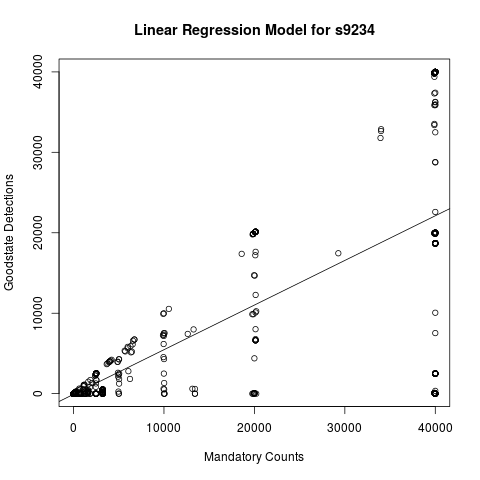
\includegraphics[scale=0.5]{Figures/s9234linereg.png}
    \end{figure}  

    The regression parameters for this model are: slope= 0.55 Intercept= -90.
    We can calculate the R-squared value by squaring $\rho$ from above, R-squared = 0.5929. 
    As was seen in the confusion matrix analysis, these values are strongly correlated, but not quite as strongly as we had hoped to see. 
    A take away from this is that while we can't really trust particular detections for circuit whose functions are unknown, we can predict about how important certain faults are relatively to one another.
    We can make this extrapolation because the regression analysis of this section is concentrated on the \textit{actual} mandatory counts, and goodstate observations.
    As opposed to the confusion matrix analysis which was only concerned about the presence of mandatory counts and goodstate observations.


    A similar analysis was performed on the DES56 circuit, and we again had more interesting results. 
    Pearson's correlation coefficient was calculated, $\rho = $ 0.88
    The linear lsregression model was plotted (Figure \ref{fig:deslinereg}).

    \begin{figure}[h!]
    \centering
    \caption{\label{fig:deslinereg}}
    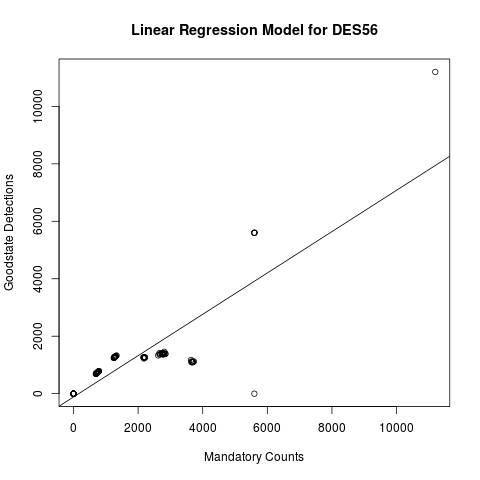
\includegraphics[scale=0.5]{Figures/deslinereg.png}
    \end{figure} 

    The regression parameters were calculated as: slope = 0.719, intercept = -116. 
    This time, we found a much higher R-squared value, which was 0.69.
    Again, we can see that when the functionality of a circuit is known, mandatory counts are a much better indicator of general fault importance. 
